La cinemática inversa es lo ``más cercano'' a nuestro mundo y a nuestra forma de actuar.
Nosotros, como seres tridimensionales, nos movemos mediante coordenadas cartesianas
conformadas por puntos definidos en los ejes $XYZ$, pero no manejamos con la misma
soltura ni facilidad las coordenadas angulares. Cuando realizamos un giro en alguna
de los brazos no lo hacemos pensando ``\textit{voy a mover el codo
15\textdegree{} a la derecha y el hombro 23\textdegree{} a la izquierda y así coloco la
mano justo donde quiero}'' sino que directamente visualizamos el movimiento que queremos 
hacer, a dónde queremos mover el brazo y sencillamente lo colocamos en esa posición,
moviendo inconscientemente las distintas articulaciones los grados necesarios.

Por esto, cuando manipulamos un brazo robótico es más sencillo indicar a dónde queremos
que vaya el \textit{end--effector} del brazo más que cúanto ha de rotar cada uno de los
motores. De esta forma, el estudio de la cinemática inversa se convierte en una de las
partes más importantes del modelo matemático de cualquier manipulador.

El problema surge en tanto que la cinemática inversa, a diferencia de la cinemática
directa, no dispone de ecuaciones que permitan obtenerla directamente. Si bien en el
punto anterior se vió cómo, a partir de una tabla de \textit{Denavit--Hartenberg},
se obtenían las matrices que permiten obtener tanto las traslaciones como las rotaciones
relativas y, al multiplicarlas, la traslación absoluta $T$ y la rotación absoluta $R$,
en la cinemática inversa no hay ningún modelo que permita una aproximación de este estilo.

A raíz de lo anterior, se plantean así dos maneras para poder obtener la relación entre
coordenadas cartesianas y coordenadas articulares:

\begin{enumerate}
    \item Mediante fuerza bruta. Como la obtención de la cinemática directa es siempre
    igual, según la precisión que se busque obtener a nivel de coordenadas cartesianas
    se puede plantear la opción de realizar un mapa de puntos: para un conjunto de
    coordenadas articulares $\left\{\theta_0^i,\theta_1^j,\cdots,\theta_n^k\right\}$ se
    obtienen unas coordenadas cartesianas 
    $\left\{x^{ij\cdots k}, y^{ij\cdots k}, z^{ij\cdots k}\right\}$ 
    (donde $i,j,\cdots,k$ representan unos ángulos en específico). 
    
    De esta manera, para el \pArm{} en específico, se tienen 
    $\left\{\theta_1, \theta_2, \theta_3\right\}$ y en total, suponiendo una precisión
    de un decimal considerando además un espectro de giro de $\left[0,180\right]\degree$,
    se disponen de una combinación de $1800^3$ posibles ángulos, lo que se traduce
    en un mapa de $\numprint{5832000000}$ ángulos que generan la misma cantidad de posiciones
    en $XYZ$. Si se quisieran usar dos decimales de precisión en ángulos (ya que hay motores capaces
    de ello), se tendrían pues $\numprint{5.832e12}$ combinaciones de ángulos y puntos.

    \item Mediante el cálculo numérico y el descubrimiento matemático. Como no hay una
    ecuación genérica que permita el cálculo de la inversa, cualquier cálculo numérico ha
    de ser previamente descubierto y estudiado. La aproximación a la cinemática inversa
    mediante este método es costosa y pueden haber situaciones en las que no resulte 
    interesante debido a la inversión en tiempo y coste: estudiar las distintas posiciones
    a las que puede llegar el manipulador, estudio de los puntos críticos del mismo
    así como plantear, si es necesario, soluciones para puntos con múltiples soluciones
    (aquellos a los que se puede llegar con combinaciones de los ángulos de entrada
    distintas).
\end{enumerate}

A la hora de desarrollar la inversa, se ha de escoger entre alguna de las dos aproximaciones
anteriores, teniendo en cuenta principalmente distintos criterios que pueden marcar la
diferencia entre uno y otro:

\begin{itemize}
    \item Por una parte, el rendimiento: el modelo matemático suele ser en general
    bastante eficiente en lo que a tiempo de cálculo se refiere, pero siempre va
    supeditado al manipulador que representa. Esto es, manipuladores con más
    grados de libertad implicaría un modelo matemático mucho más complejo que según
    las operaciones que implique puede no ser viable para el sistema en que se va a ejecutar.

    Por su lado, un mapa por su estructura y organización siempre permite el acceso a las
    claves y sus valores bajo un $\bigO{1}$, haciéndolos la mejor opción en términos
    de eficiencia si se busca una ejecución rápida.

    \item Por otra, la memoria: un mapa siempre requiere de mucha más memoria que 
    una primitiva u otra estructura de datos. Principalmente se debe a su organización
    en memoria ya que, además de las claves y sus valores, se debe guardar un \textit{hash}
    o un \textit{set} (según esté implementada la librería) de todas y cada una de las 
    claves, para garantizar así que el tiempo de acceso sea $\bigO{1}$.
    Además, el mapa tendría que ir guardado o directamente en el espacio de código
    (y copiado a la \ac{RAM} en tiempo de ejecución) o bien guardado en un fichero
    binario que permitiese su posterior carga en el sistema, lo cual implica que sería
    necesario contar con ese espacio en el sistema de ficheros donde se guarde.

    En cambio, el modelo matemático carece de este problema ya que se utilizan
    principalmente primitivas y operaciones matemáticas que se realizan directamente
    sobre un co-procesador, si existe, o sobre el procesador en sí. Aunque se puedan
    usar muchas primitivas, es difícil que alcancen en tamaño en memoria a un mapa.

    \item Además, hay que tener en cuenta el esfuerzo de la obtención. La aproximación
    por fuerza bruta requiere de bastante tiempo para la obtención del mapa al completo,
    y un cambio en la cantidad de decimales implicaría un recálculo casi completo del mapa
    con un aumento de tiempo exponencial, pero se podría dejar automatizado y que se realice
    automáticamente por otro equipo.

    Sin embargo, dado que el modelo matemático requiere de un descubrimiento y estudio
    de tanto las características geométricas del manipulador como de las interacciones
    entre los elementos del mismo, el tiempo es en principio desconocido. Según el nivel
    de las personas trabajando en ello puede ser mayor o menor, pero luego la verificación
    y comprobación del mismo puede implicar tener que replantearlo y modelarlo de nuevo.
\end{itemize}

Para este proyecto se ha preferido hacer el modelo matemático, ya que se plantearon las
características del modelo por fuerza bruta pero fue descartado ya que se estimaba un
uso de memoria excesivo (no habría cabido en el dispositivo\footnote{teniendo en cuenta
que habría sido necesario guardar tuplas de tres elementos por clave junto con tuplas de
otros tres elementos para el valor, donde cada elemento sería de tipo \texttt{float}
(lo que se traduce en \textit{4 bytes} por elemento), habría supuesto un uso de 
aproximadamente $\left(\numprint{5.382e9}\right)^2 \cdot \numprint[B]{4} = \numprint[B]{1.158e20} \approx \numprint[TB]{1.158e11} $,
lo cual es inviable para el sistema.}). Además, dado que se cuenta con un procesador
con gran capacidad de cómputo las operaciones matemáticas se realizan a una gran velocidad,
en particular las multiplicaciones ya que se cuenta con un conjunto de instrucciones y
con una \ac{ALU} que permiten realizarlas a la misma velocidad que una suma con números de hasta
16 bits \cite{microchipDsPIC33EPIC24EFRM2010}.

Para plantear la cinemática inversa del \pArm{} hay que distinguir dos partes:
\begin{itemize}
    \item La base $\left(\theta_0\right)$, que rota sobre el eje $Y$ y cuyo movimiento no está supeditado al
    del resto de motores.

    \item El triángulo superior, conformado por $\left\{\theta_1, \theta_2\right\}$ donde
    los ambos ángulos dependen de la posición final y están directamente relacionados.
\end{itemize}

Por otra parte, dada la configuración geométrica del robot, sabemos las siguientes premisas:

\begin{itemize}
    \item $x$ se encuentra comprendido en el rango $\left(0, A_{M_L}\right]$, donde $A_{ML}$
    es ``\textit{Arm Maximum Length}'' y viene definido por la ecuación \ref{eq:aml}:

    \begin{equation}\label{eq:aml}
        A_{M_L} = \left(\overline{A_L} + \overline{A_U}\right) \cdot \cos{\theta^{LU}_{Max}} + A_{EF_L}\\
    \end{equation}

    donde cada uno de los elementos anteriores representan:

    \begin{equation*}
        \left\{\begin{aligned}
            \overline{A_L} & \equiv \text{``\textit{Arm Lower}''} = \numprint[mm]{142} \\
            \overline{A_U} & \equiv \text{``\textit{Arm Upper}''} = \numprint[mm]{158.8} \\
            \theta^{LU}_{Max} & \equiv \widehat{A_L A_U}_{Max} = \frac{13\pi}{15}~rad \\
            A_{EF_L} & \equiv \text{``\textit{Arm End--Effector Length}''} = \numprint[mm]{44.5} \\
        \end{aligned}
        \right.
    \end{equation*}

    \item $y$ por su parte se encuentra comprendido en el rango $\left[-A_{M_L}, A_{M_L}\right]$,
    donde $A_{M_L}$ está definido en la ecuación anterior (ecuación \ref{eq:aml}).
    \item $z$ pertenece al rango $\left[0, A_{M_H}\right]$, donde $A_{M_H}$ es 
    ``\textit{Arm Maximum Height}'' y viene definido por la ecuación \ref{eq:amh}:
    
    \begin{equation}\label{eq:amh}
        A_{M_H} = A_{B_H} + \overline{A_L} + \overline{A_U} \cdot \sin{^{Max}\theta^{A_U}_{A_L \parallel A_B}}
    \end{equation}

    donde los elementos anteriores representan:
    \begin{equation*}
        \left\{\begin{aligned}
            A_{B_H} & \equiv \text{``\textit{Arm Base Height}''} = \numprint[mm]{106.1} \\
            ^{Max}\theta^{A_U}_{A_L \parallel A_B} & \equiv \text{``Ángulo máximo de $A_U$ cuando $A_L \parallel A_B$''} = \frac{\pi}{8}~rad \\
        \end{aligned}
        \right.
    \end{equation*}
\end{itemize}

De esta forma, tenemos que:

\begin{align*}
    x & \in \left(0, A_{M_L}\right] \\
    y & \in \left[-A_{M_L}, A_{M_L}\right] \\
    z & \in \left[0, A_{M_H}\right] \\
\end{align*}


, dada la configuración geométrica del
mismo, se parte de un triángulo que relaciona la parte superior del brazo (ver figura
\ref{fig:ik_pArm_triangle}).

\begin{figure}
    \centering
    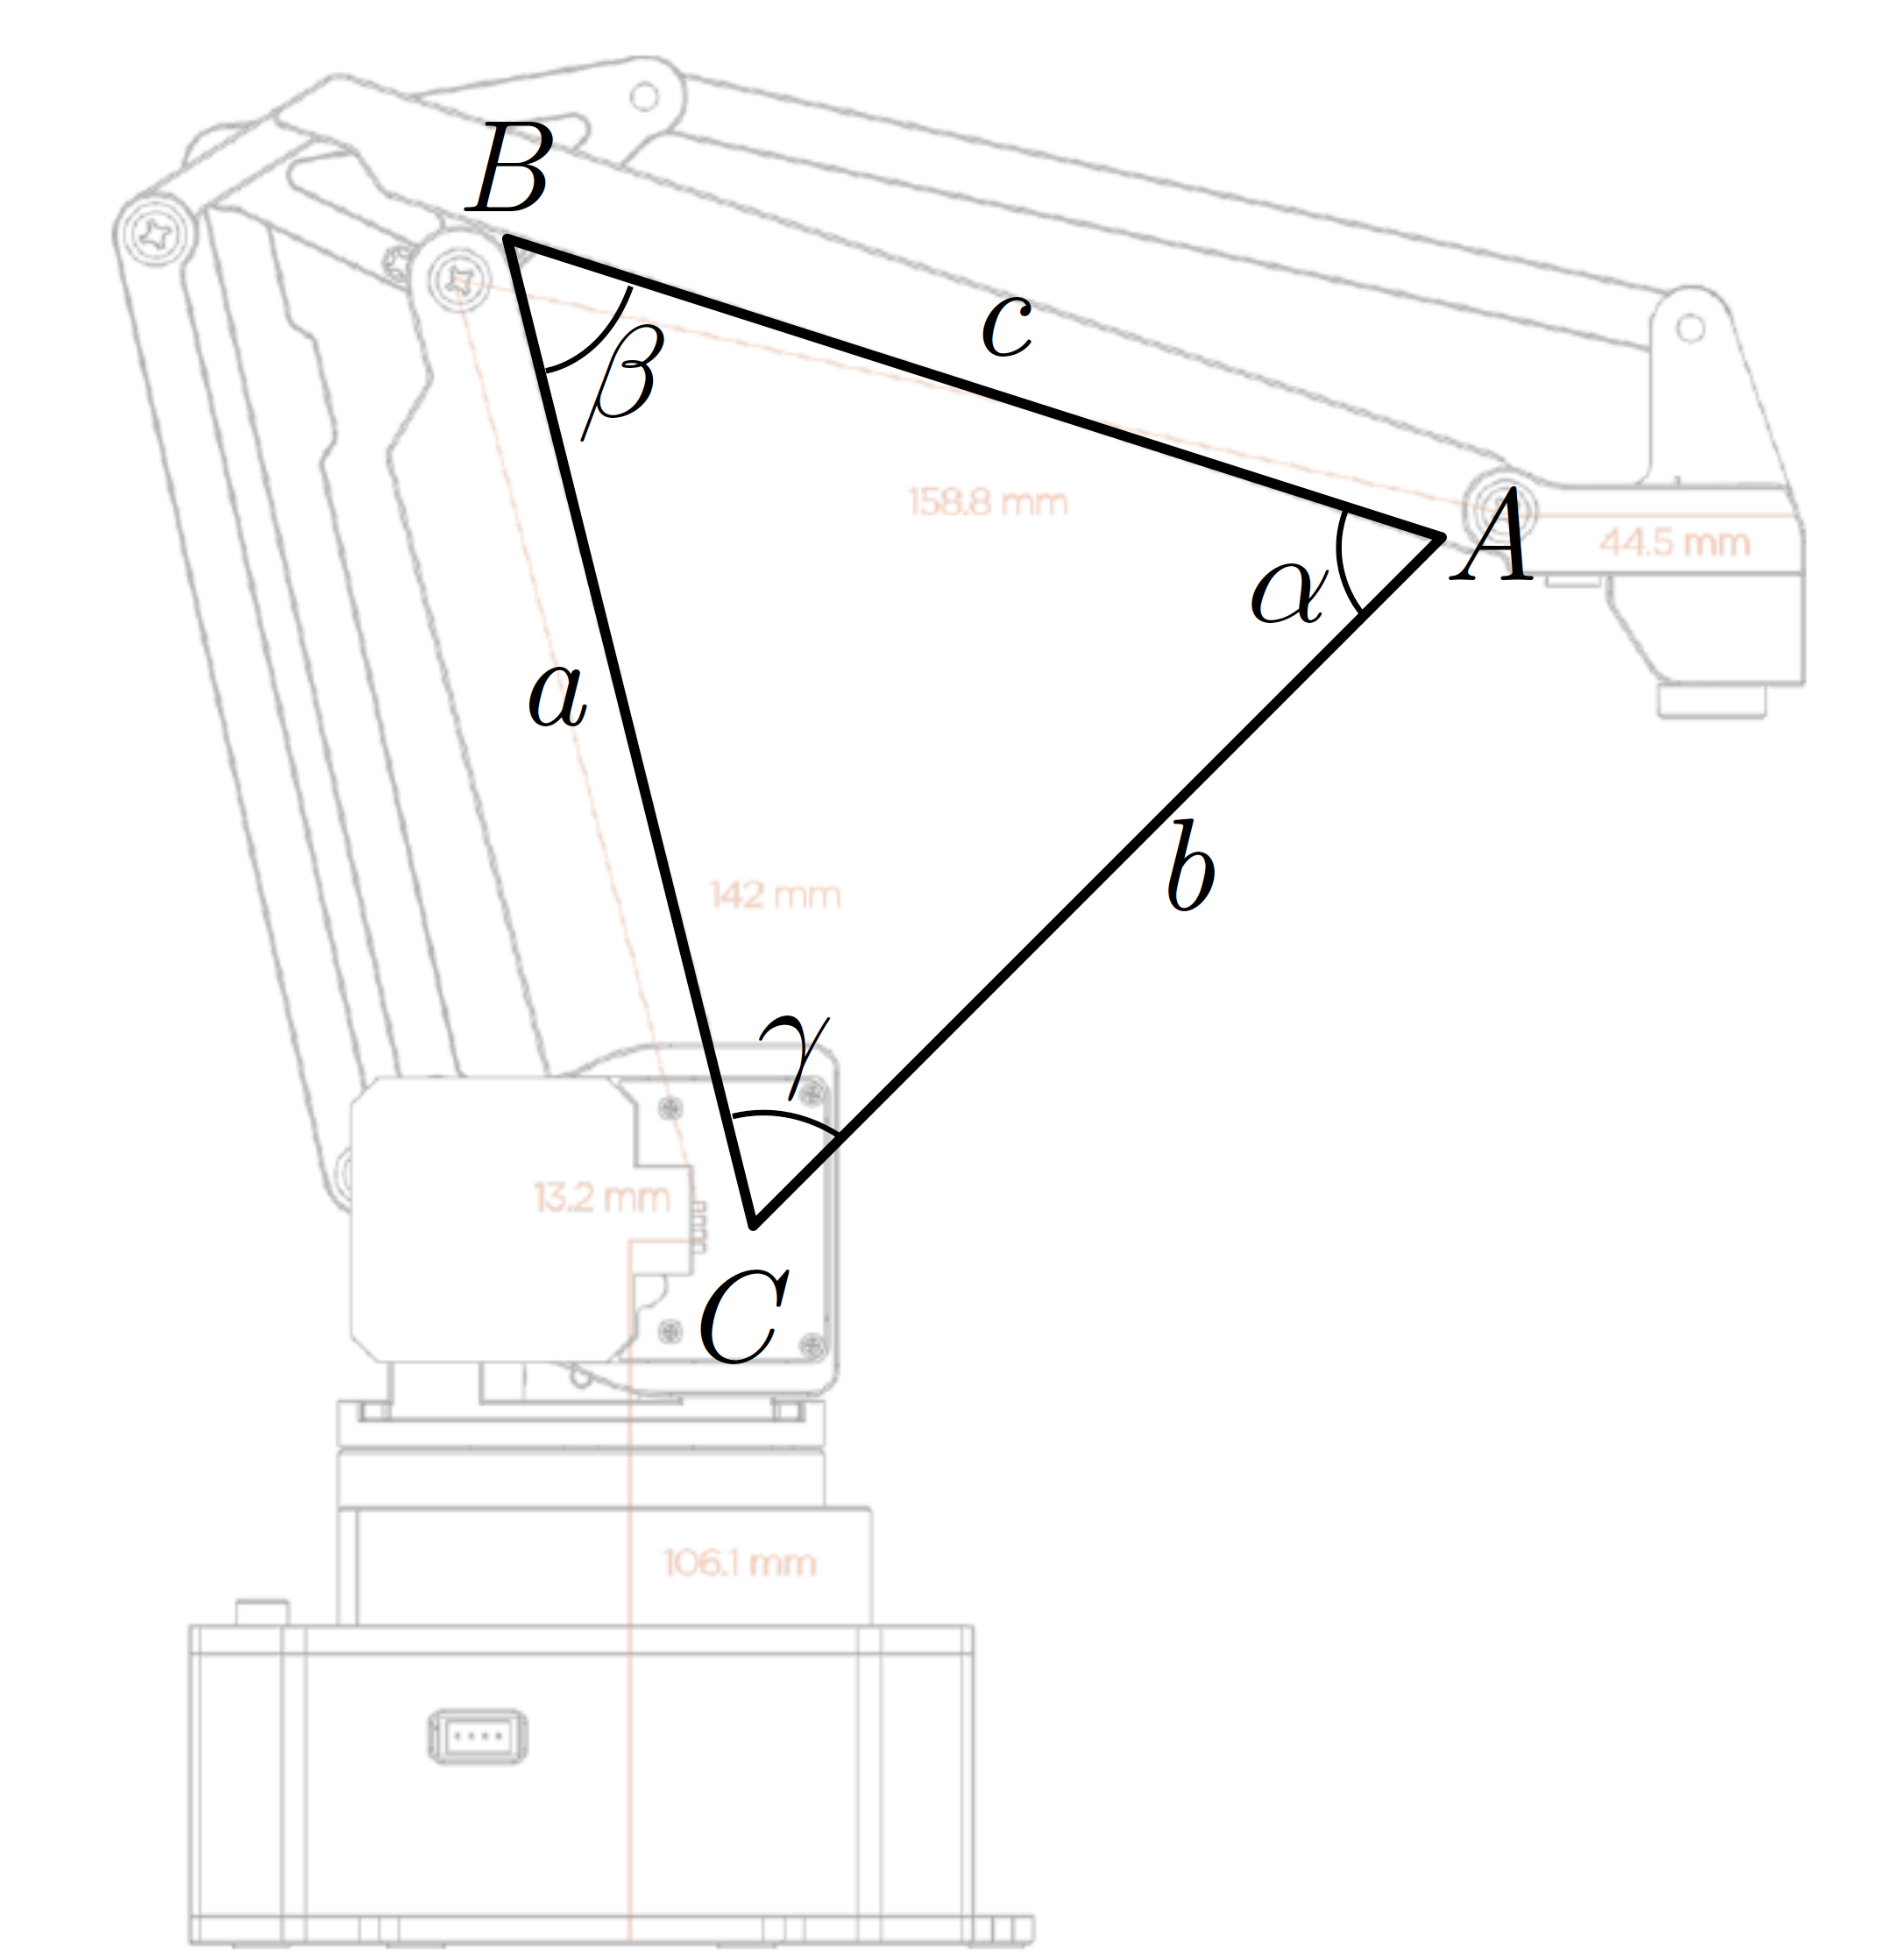
\includegraphics[width=.7\linewidth]{pictures/ik_cosine_law_over_arm.png}
    \caption{Aproximación para la cinemática inversa de la parte superior del brazo.}
    \label{fig:ik_pArm_triangle}
\end{figure}